\pdfoutput=1
\pdfcompresslevel=9
\pdfinfo
{
    /Author (M.Lis)
    /Title (BachelorThesis)
    /Subject (NASA Voyager 1 space mission risk assessment)
    /Keywords (risk assessment)
}
\documentclass[a4paper,onecolumn,oneside,11pt]{report}
\usepackage[utf8]{inputenc}
\usepackage[sfdefault]{arimo}
\usepackage[T1]{fontenc}
\usepackage{textcomp}
\usepackage[a4paper, total={6in, 8in}]{geometry}
\usepackage[english]{babel}
\usepackage{setspace}
\usepackage{biblatex}
\usepackage{amsmath}
\usepackage{graphicx} % pakiet do zamieszczanie garfiki
\usepackage{caption}
\usepackage{acro}
\usepackage[final]{pdfpages}
\usepackage{lscape} 
\usepackage{array}% pakiet do dodawania paddingu w tabelach
\newcolumntype{L}[1]{>{\raggedright\let\newline\\\arraybackslash\hspace{0pt}}m{#1}}
\newcolumntype{C}[1]{>{\centering\let\newline\\\arraybackslash\hspace{0pt}}m{#1}}
\newcolumntype{R}[1]{>{\raggedleft\let\newline\\\arraybackslash\hspace{0pt}}m{#1}}
\usepackage{makecell} % pakiet do newline w tabeli
\usepackage{csquotes}

\usepackage{titlesec}
\titleformat{\chapter}{\huge}{\thechapter.}{20pt}{\huge\it}%do suuniecia slowa chapter

\addbibresource{sample.bib}

% probably a good idea for the nomenclature entries:
\acsetup{first-style=short}

\addto\captionenglish{
  \renewcommand{\contentsname}
    {Table of Contents}%
    }

\hyphenpenalty=10000		% nie dziel wyrazów zbyt często
\clubpenalty=100000		% kara za sierotki
\widowpenalty=10000			% nie pozostawiaj wdów
\brokenpenalty=10000		% nie dziel wyrazów między stronami
\exhyphenpenalty=999999		% nie dziel słów z myślnikiem
\righthyphenmin=3			% dziel minimum 3 litery

\tolerance=4500
\pretolerance=250
\hfuzz=1.5pt
\hbadness=1450

\sloppy						% umacnia pozycję prawego marginesu

\setlength{\textwidth}{\paperwidth}
\addtolength{\textwidth}{-5cm}
\setlength{\textheight}{\paperheight}
\addtolength{\textheight}{-5cm}
\setlength{\oddsidemargin}{0cm}
\setlength{\evensidemargin}{0cm}
\topmargin -1.25cm
\footskip 1.5cm
\linespread{1.3} %przerwy miedzy wierszami

\begin{document}


\includepdf[pages=-]{first_page.pdf}

% \begin{titlepage}
% 	\begin{center}
	
% 	\begin{figure}[h] % h od here
% \centering
% 
\includegraphics[scale=0.75]{images/logo_pw.png}
% \end{figure}
	
% 	\vspace*{2\baselineskip}
% 	\fontseries{m}\fontsize{32pt}{20pt}\selectfont
% 	Praca dyplomowa \\inżynierska\\
% 	\vspace*{0.5\baselineskip}
% 	\fontsize{15pt}{15pt}\selectfont
% 	na kierunku Lotnictwo i Kosmonautyka\\
% 	w specjalności Automatyka i Systemy Lotnicze\\
% 	\vspace*{1.15\baselineskip}
% 	\fontseries{b}\fontsize{15pt}{18pt}\selectfont
% 	NASA Voyager 1 space mission risk assessment\\
% 	\vspace*{1.15\baselineskip}
% 	\fontsize{22pt}{15pt}\selectfont
% 	Michał Lis\\
% 	\fontsize{15pt}{15pt}\selectfont
% 	\vspace*{0.25\baselineskip}
% 	Numer albumu 271299\\
% 	\fontsize{15pt}{15pt}\selectfont
% 	\vspace*{1\baselineskip}
% 	Promotor\\prof. nzw. dr hab. inż. Marek Matyjewski\\
% 	\end{center}

% 	\vspace*{8.5\baselineskip}
% 	\begin{flushright}
% 	\fontseries{m}\fontsize{13pt}{10pt}\selectfont
% 	\end{flushright}
% 	\begin{center}
% 	Warszawa, 2018
% 	\end{center}
% \end{titlepage}


\begin{center}
\textbf{Summary}
\end{center}

Voyager Space mission is one of the longest lasting scientific programs run by National Aeronautics and Space Administration. It employs two robotic probes to explore giant planets of our Solar System like Jupiter, Saturn, Uranus and Neptune and the interstellar medium beyond the borders of heliosphere. The mission took great advantage of a favourable planetary alignment that enabled gravitational assists of these giant planets. After exploration of Jupiter and Saturn, one of the spacecrafts, Voyager1, headed towards the heliopause to examine the characteristics of the medium outside of our Solar System. Its mission is still continuing and thus Voyager 1 is the farthest still-operating human-made object sent into outer space. Although not all of the science instruments on-board are operating, it can still communicate and transmit some data to Deep Space Network. It is predicted that it will run out of energy and end its task around 2025.

The definition of risk in terms of space missions, according to Christian Preyssl, European Space Agency risk assessment specialist involve the events that are "introduced by potential problem situations in a project that have undesirable consequences in terms of cost, schedule, and technical performance". Taking into consideration Voyager mission's date of realization, very long execution time and extraordinary mission's profile the program was fraught with certain risk of failure. As Voyager's were launched in 1970s, the technical documentation for the mission and space probes is available to public, what enabled the author to acquire more detailed information and carry out this risk assessment procedure. Such a calculation could be carried out in many different ways. In the following bachelor thesis titled "NASA Voyager 1 space mission risk assessment" the method used is a simplified scheme developed for estimating the risk of student satellite projects, which is based on Likelihoods-Consequence matrix.

The first part of this work focuses on describing the mission's historical context, profile, requirements and the main obstacles that the space probe had to overcome. In the next part I describe the technical solutions employed in Voyager's construction and, taking advantage of technical documentation of the spacecraft, I try to find the strong and weak points in the design. Then I present the history of risk management at NASA as well as the Agency's currently implemented methodology. The following chapter is the main goal of this work - experimental mission risk assessment using the simplified L-C method: identification of root causes for each risk, estimation of Likelihood and Consequence coefficients, validation of its values and creation of the on L-C chart. Finally, some risk mitigation techniques are proposed and as a summary of this work the conclusions from the conducted risk assessment are presented.

\vspace*{\baselineskip}

\noindent\textbf{Keywords:} \textit{Risk, risk assessment, risk analysis, space mission, NASA, Voyager, risk management.}
\newpage

\begin{center}
\textbf{Streszczenie}
\end{center}

Program Voyager jest obecnie jednym z najdłużej trwających kosmicznych programów badawczych prowadzonych przez amerykańską organizację National Aeronautics and Space Administration, w ramach którego w 1977 roku wystrzelono dwie bezzałogowe sondy kosmiczne w celu zbadania czterech gazowych olbrzymów (Jowisza, Saturna, Urana i Neptuna). Korzystając z optymalnej wzajemnej konfiguracji zewnętrznych planet naszego układu, która umożliwiła skorzystanie z dużej liczby asyst grawitacyjnych, sonda Voyager 1 miała dokonać eksploracji układów Jowisza i Saturna. Następnie po zakończeniu badania tych planet, główne zadanie stanowić miała eksploracja krańcowych obszarów heliosfery, przekroczenie heliopauzy oraz pomiar właściwości przestrzeni międzygwiezdnej. Obecnie misja Voyagera 1 wciąż trwa, a sonda ta stanowi najdalszy i ciągle działający obiekt wysłanym w przestrzeń kosmiczną przez człowieka. Pomimo że nie wszystkie instrumenty badawcze znajdujące się na jej pokłądzie funkcjonują prawidłowo, sonda nadal komunikuje się ze stacjami Deep Space Network. Przewiduje się, że zasilanie w energię elektryczną wystarczy do utrzymania funkcjonowania i łączności z Ziemią do około 2025 roku.

Definicja ryzyka w odniesieniu do projektów kosmicznych przytoczona przez Christiana Preyssl'a, specjalisty European Space Agency do spraw ryzyka to "potencjalne wydarzenia, które powodują niepożądane konsekwencje z punktu widzenia kosztów, terminarza i osiągów technicznych". Biorąc pod uwagę czas wykonania, bardzo długi okres realizacji a także charakter projektu, program Voyager obarczony był pewnym ryzykiem niepowodzenia. Ze względu na fakt, że misja została opracowana w latach siedemdziesiątych jej dokumentacja techniczna jest publicznie dostępna, co pozwoliło autorowi pracy na przeprowadzenie owej analizy ryzyka. Taka analiza może odbywać się na wiele sposobów. Niniejsza praca pt. ,,NASA Voyager 1 space mission risk assessment'' wykorzystuje uproszczoną metodę opierającą się na macierzy ryzyka Likelihood-Consequence. 

Pierwsza część pracy to opis kontekstu historycznego misji, jej program, zadania naukowe a także wyzwania z którymi sonda musiała się zmierzyć. W następnej części dokonano przeglądu technicznych rozwiązań zastosowanych podczas projektowania Voyager'a 1, a także, posługując się dokumentacją techniczną sondy, wypunktowano jej silne i słabe strony. Następnie dokonano przeglądu metodologii stosowanych do zarządzania ryzykiem w NASA, podkreślając przy tym współczesne metodyki. Kolejny etap to już główna część pracy - eksperyment polegający na analizie ryzyka misji uproszczoną metodą L-C: zidentyfikowanie przyczyn potencjalnych zagrożen, oszacowanie współczynników prawdopodobieństwa i konsekwencji oraz naniesie ich wartości na macierz L-C. Na koniec zaproponowane zostały techniki minimalizacji ryzyka oraz zaprezntowane zostało podsumowanie pracy - wnioski wyciągnięte z przeprowadzonej analizy ryzyka misji Voyager'a.

\vspace*{\baselineskip}

\noindent\textbf{Słowa kluczowe:} \textit{Ryzyko, analiza ryzyka, misja kosmiczna, NASA, Voyager, zarządzanie ryzykiem.}
\newpage



% \begin{center}
%     \fontsize{15pt}{15pt}\selectfont
% Oświadczenie autora pracy
% \vspace*{1.15\baselineskip}
% \end{center}

% Świadom odpowiedzialności prawnej oświadczam, że przedstawiona praca
% dyplomowa:\\
% - została napisana przeze mnie samodzielnie i nie zawiera treści uzyskanych w
% sposób niezgodny z obowiązującymi przepisami,\\
% - nie była wcześniej przedmiotem procedur związanych z uzyskaniem tytułu
% zawodowego lub stopnia naukowego w wyższej uczelni.\\
% Oświadczam ponadto, że niniejsza wersja pracy jest identyczna z załączoną wersją
% elektroniczną.\\
% \vspace*{1.15\baselineskip}
% \noindent\begin{tabular}{ll}
% \makebox[2.5in]{\hrulefill} & \makebox[2.5in]{\hrulefill}\\
% data & podpis autora (autorów) pracy\\[8ex]% adds space between the two sets of signatures
% \end{tabular}

% \begin{center}
%     \fontsize{15pt}{15pt}\selectfont
% Oświadczenie
% \vspace*{1.15\baselineskip}
% \end{center}

% Wyrażam zgodę / nie wyrażam zgody na udostępnianie osobom zainteresowanym
% mojej pracy dyplomowej. Praca może być udostępniana w pomieszczeniach
% biblioteki wydziałowej. Zgoda na udostępnienie pracy dyplomowej nie oznacza
% wyrażenia zgody na jej kopiowanie w całości lub w części.
% Brak zgody nie oznacza ograniczenia dostępu do pracy dyplomowej osób:\\
% - reprezentujących władze Politechniki Warszawskiej,\\
% - członków Komisji Akredytacyjnych,\\
% - funkcjonariuszy służb państwowych i innych osób uprawnionych, na mocy
% odpowiednich przepisów prawnych obowiązujących na terenie Rzeczypospolitej
% Polskiej, do swobodnego dostępu do materiałów chronionych międzynarodowymi
% przepisami o prawach autorskich. Brak zgody nie wyklucza także kontroli tekstu
% pracy dyplomowej w systemie antyplagiatowym.\\
% \vspace*{1.15\baselineskip}
% \noindent\begin{tabular}{ll}
% \makebox[2.5in]{\hrulefill} & \makebox[2.5in]{\hrulefill}\\
% data & podpis autora (autorów) pracy\\[8ex]% adds space between the two sets of signatures
% \end{tabular}
% \newpage

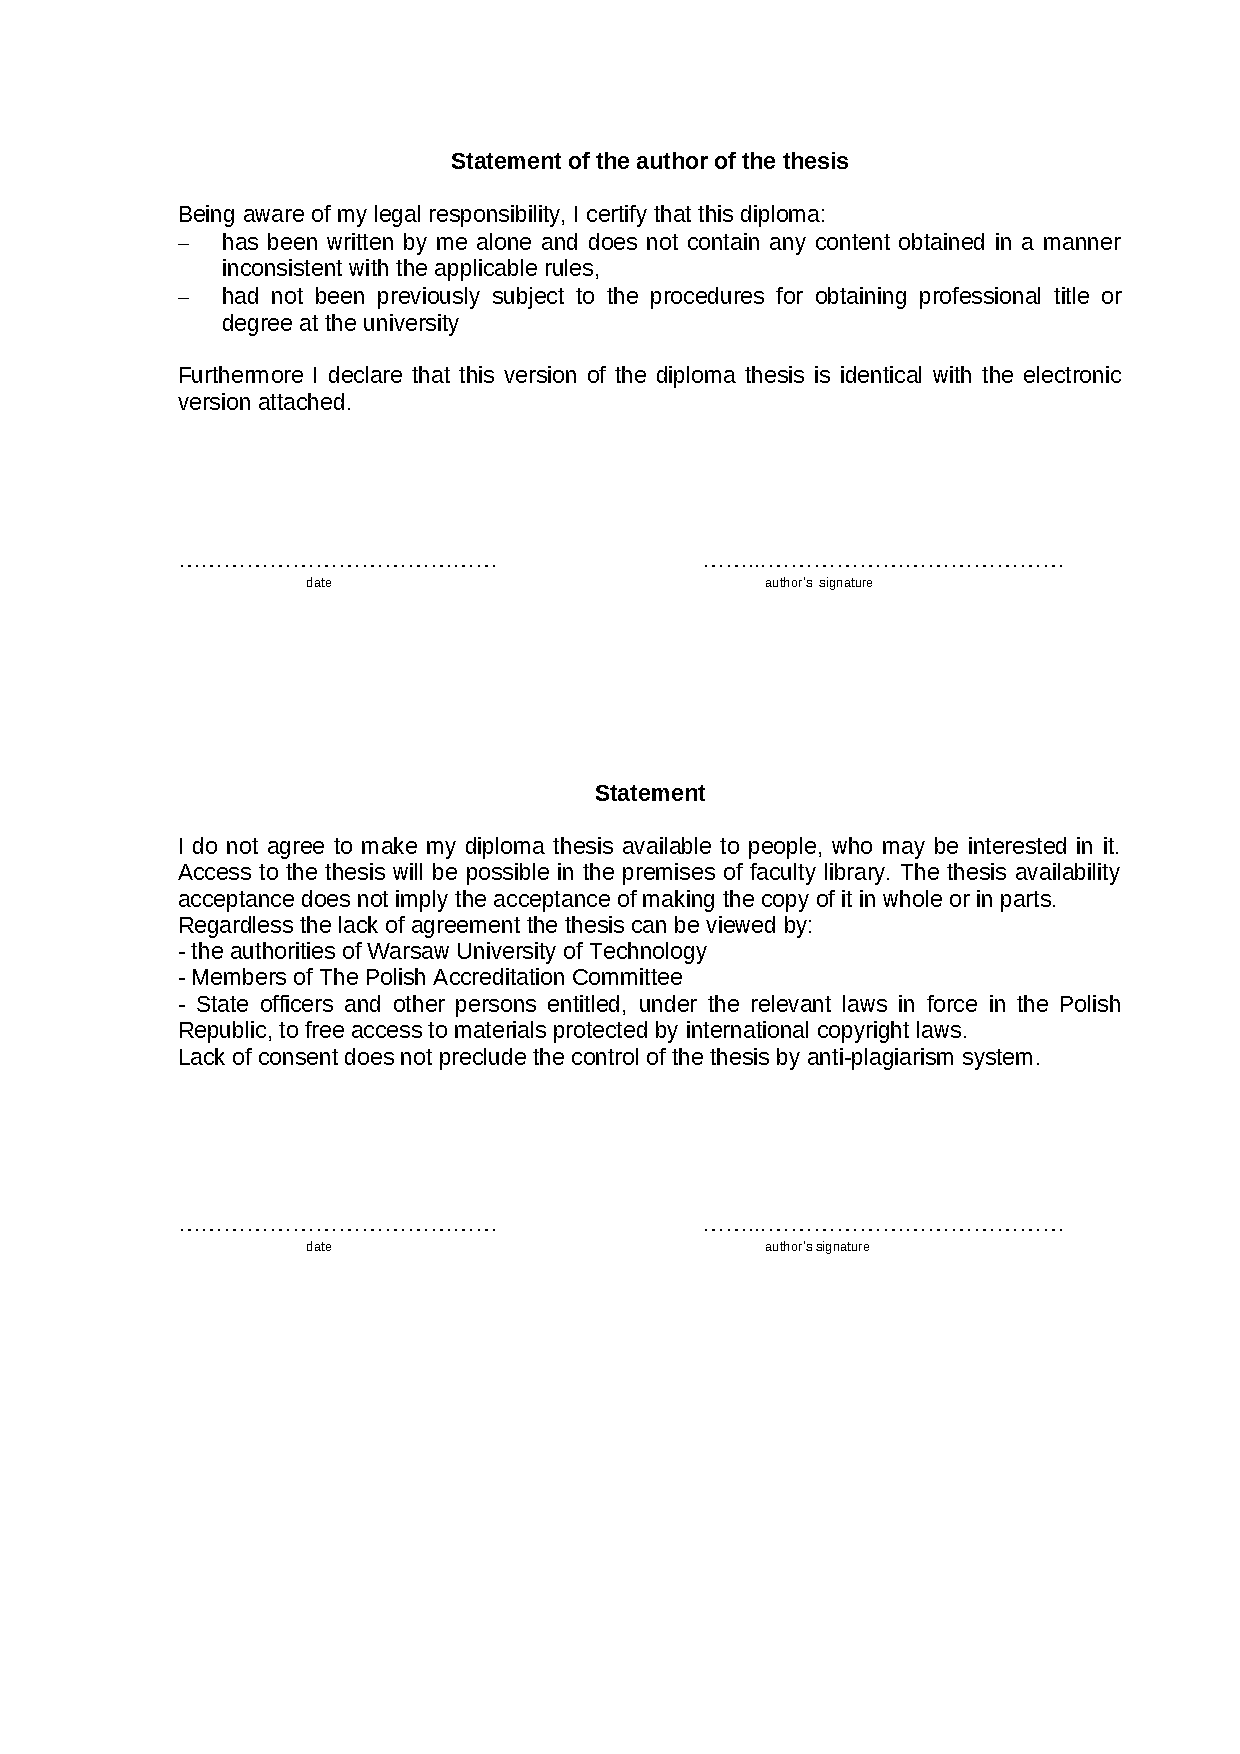
\includepdf[pages=-]{fourth_page.pdf}

\tableofcontents

\chapter{Introduction}
ble ble ble
\chapter{Voyager Mission overview}
\section{Mission on the NASA timeline}
ble ble ble
\chapter{Voyager 1 spacecraft design}

\section{General design idea}
ble ble ble
\chapter{Mission risk assessment}
\section{Overview of risk management methods for space missions}
ble ble ble
\section{L-C method implementation}

The risk mission assessment presented in this work will follow the L-C method steps specified in the table 4.1 from the previous subsection. In order to understand the requirements of the program based on NASA standards and which mission-specific actions could cause failure, some other space mission risk case studies were analyzed, including a report "Risk Management for the NASA/JPL Genesis Mission: A Case Study" published by NASA \cite{genesis}, a case study of the ARMADILLO satellite presented in the document by Brumbaugh \cite{Brumbaugh} and "Report on Project Management in NASA" produced by the Mars Climate Orbiter Mishap Investigation Board in order to maximize the possibility of success for future similar missions \cite{mro}.

\subsection{Mission concept review and identification of risk categories}
\chapter{Conclusions}

ble ble ble

\printbibliography
\clearpage

\begin{table}[h]
    {\huge \textit{List of Acronims}}
    \begin{center}
        \begin{tabular}{ L{4cm} L{10cm}}
             \\ \\ \\
            NASA & National Aeronautics and Space Administration \\ \\
            
            ESA & European Space Agency \\ \\
            
            L-C & Likelihoods-Consequence \\ \\
            
            PRA & Probabilistic Risk Assessment \\ \\
            
            JPL & Jet Propulsion Laboratory \\ \\
            
            PGT & Planetary Grand Tour \\ \\
            
            DSN & Deep Space Network \\ \\
            
            FDS & Flight Data Subsystem \\ \\
            
            AACS & Attitude and Articulation Control Subsystem \\ \\
            
            CCS & Computer Command Subsystem \\ \\
            
            DSS & Data Storage System \\ \\
            
            RTG & Radioisotope Thermoelectric Generators \\ \\
            
            ISS & Imaging Science System \\ \\
            
            IRIS & Infrared Interferometer-Spectrometer and Radiometer \\ \\
            
            UVS & Ultraviolet Spectrometer \\ \\
            
            PS & Photopolarimeter Subsystem \\ \\
            
            RSS & Radio Science System \\ \\
            
            PRAS & Planetary Radio Astronomy \\ \\
            
            PWS & Plasma Wave Subsystem \\ \\
             
            CRS & Cosmic Ray System \\ \\
            
            RM & Risk Management \\ \\
            
            CRM & Continuous Risk Management \\ \\
        \end{tabular}
            \label{table:30}
    \end{center}
\end{table}


\clearpage
\clearpage

\begin{table}[h]
    \begin{center}
        \begin{tabular}{ L{4cm} L{10cm}}
            
            OSMA & Office of Safety and Mission Assurance \\ \\
            
            RIDM & Risk Informed Decision Making \\ \\
            
            L-C Chart & Likelihood Consequence Chart \\ \\
            
            LC & Likelihood Consequence Method \\ \\
            
            LAU & Launch risk category \\ \\
            
            SCI & Science risk category  \\ \\
            
            COMM & Communication risk category  \\ \\
            
            SPA & Space Probe risk category \\ \\
            
            MTN & Maintenance risk category \\ \\
            
            SCH & Schedule risk category \\ \\
            
            RR & Rank Reciprocal \\ \\
            
            ROC & Rank Order Centroid \\ \\
            
            RS & Rank Sum \\ \\
            
            EW & Equal Weights \\ \\
            
        \end{tabular}
            \label{table:30}
    \end{center}
\end{table}


\clearpage
\listoffigures
\listoftables
\addcontentsline{toc}{chapter}{\protect\numberline{}Bibliography}
\addcontentsline{toc}{chapter}{\protect\numberline{}List of used symbols and abbreviations}
\addcontentsline{toc}{chapter}{\protect\numberline{}List of figures}
\addcontentsline{toc}{chapter}{\protect\numberline{}List of tables}
\addcontentsline{toc}{chapter}{\protect\numberline{}Appendices}
\cleardoublepage

\nocite{*}


\end{document}
